%\chapter{Vorlesung}
%\section{Binärer Suchbaum}
\pagebreak
\begin{figure}[H]
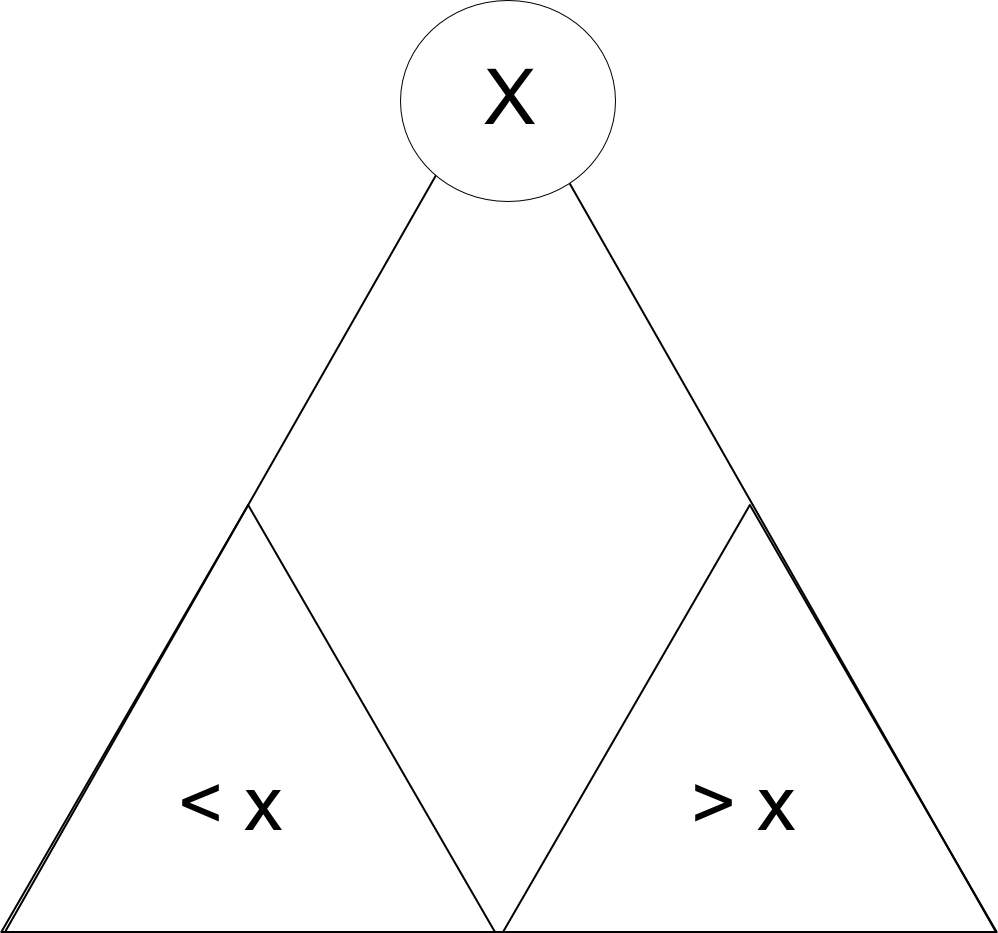
\includegraphics[width=0.2\linewidth]{10/Grafik/img1.png}
\captionsetup{justification=raggedright, singlelinecheck=false}
\caption{Binärer Suchbaum}
\end{figure}

\section{Pseudo-Code}
\lstinputlisting[language=Java, style = pseudo]{10/Code/Node.java}


\chapter{AVL-Bäume von Adelson-Velsky and Landis}%Ursprünglich nur AVL-Bäume, Ergänzung von Markus
\section{Allgemein} %Ergänzung von Markus
\paragraph{Ziel}Binärer Suchbaum mit garantierter Such-, Einfüge- und Löschzeit $O(\log n )$
\paragraph{Idee} Definiere eine Balancebedingung, die dafür sorgt, dass die Baumstruktur möglichst nahe an der Idealstruktur eines vollständigen binären Baumes liegt.\\
Aber gleichzeitig soll es möglich sein ''schnell'' Strukturänderungen beim Einfügen und Löschen vorzunehmen. \\

\begin{figure}[H]
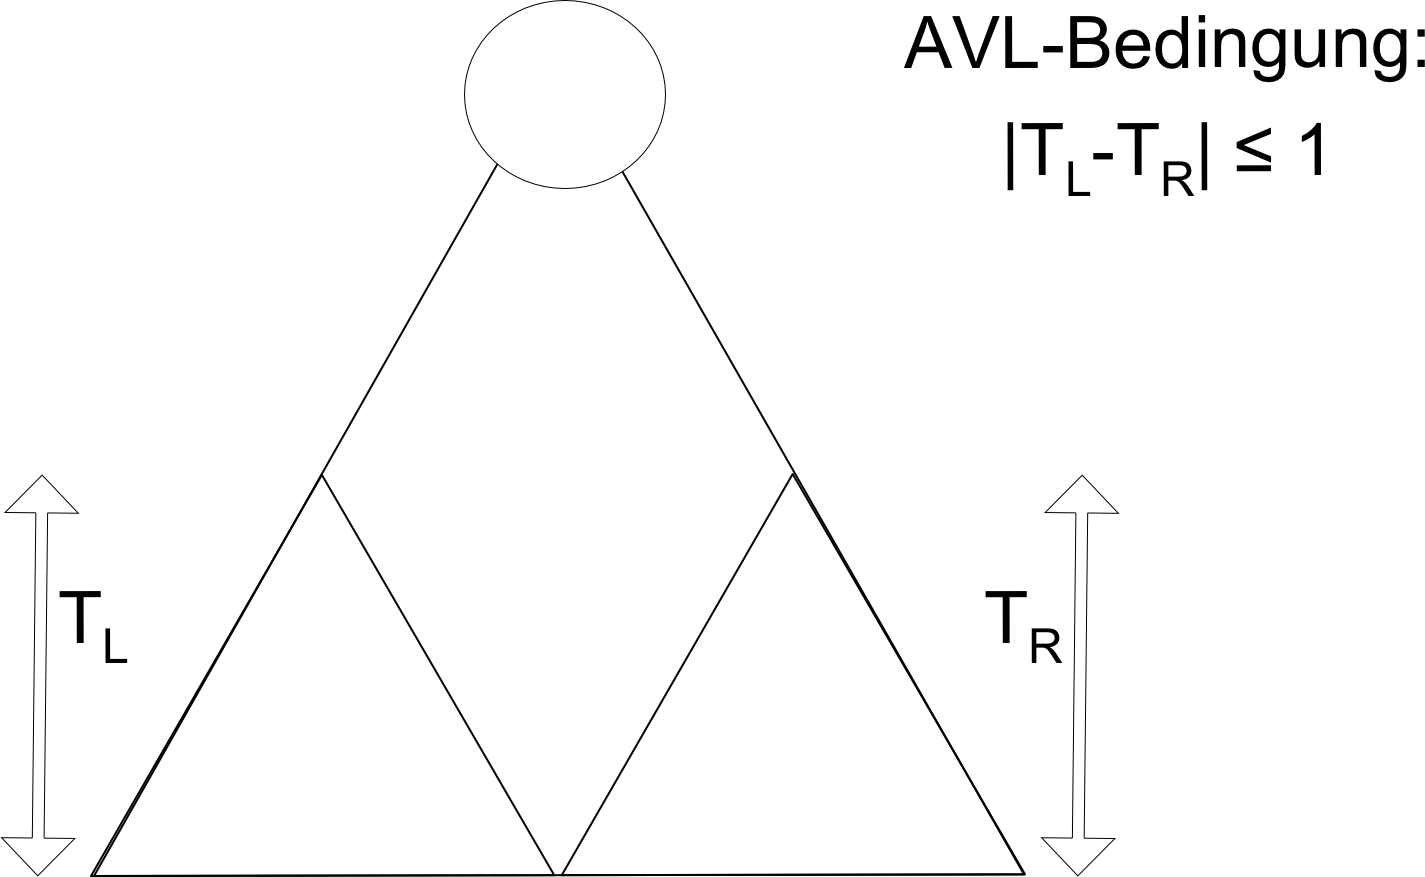
\includegraphics[width=0.4\linewidth]{10/Grafik/img2.png}
\captionsetup{justification=raggedright, singlelinecheck=false}
\caption{AVL-Baum}
\end{figure}


\section{Laufzeitanalyse}
\paragraph{Ziel} Analyse der erwarteten maximalen Tiefe randomisierter binärer Suchbäume \\

Sei der Schlüssel der Wurzel das i-kleinste Element \\

\begin{wrapfigure}[2]{l}{0.3\linewidth}
	\vspace{-50pt}
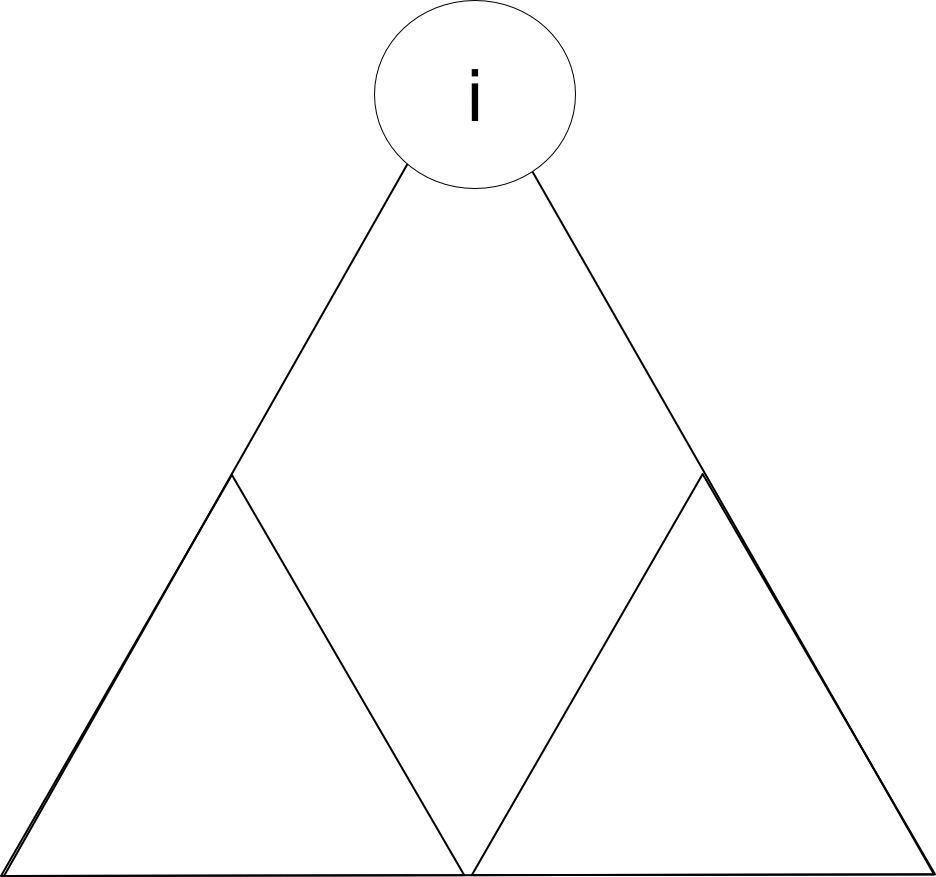
\includegraphics[width=\linewidth]{10/Grafik/img3.png}
\noindent i-1 Elemente \hfill \hfill m-i Elemente
\caption{}
\end{wrapfigure}

\vspace{30pt}
$T_n ~\hat{=}~$ maximale Tiefe eines randomisierten Suchbaums mit $\{1,...,n\}$ Elementen\\
\vspace{50pt}


\pagebreak

\subsection*{}
\textbf{Für den Fall, dass i als Wurzelknoten gewählt wird gilt:}
\[T_n=max\{T_{i-1}, T_{n-i}\}+1\]
\[X_n = 2^{T_n} ~ \text{exponentielle Tiefe}\]
\[2^{T_n} = 2^{1+max\{T_{i-1}, T_{n-1}\}} = 2 \cdot 2^{max\{T_{i-1}, T_{n-1}\}} = 2 \cdot max\{2^{T_{i-1}}, 2^{T_{n-1}}\}\]
\[\Rightarrow X_n = 2 \cdot max\{X_{i-1}, X_{n-1}\} \] \\

\textbf{Mit der Abschätzung: $max\{2^{T_1}, 2^{T_2}\} \leq 2^{T_1} + 2^{T_2}$ folgt:}
\[E(X_n) = E \left(\sum^n_{i=1} \frac{1}{n} \cdot  2 \cdot max\{X_{i-1}, X_{n-1}\} \right) \]
\[= \frac{2}{n} \sum^n_{i=1} E \left(max\{X_{i-1}, X_{n-1}\} \right) \leq \frac{2}{n} \sum^n_{i=1} E \left(X_{i-1} + X_{n-1} \right) \]
\[=\frac{2}{n} \sum^n_{i=1} \left[E(X_{i-1}) + E(X_{n-i}) \right] \leq \frac{4}{n} \sum^{n-1}_{i=0} E(X_i)\] 

\[ n \cdot E(X_n) = 4 \cdot \sum^{n-1}_{i=0} E(X_i) ~~~(1)\]
\[ (n-1) \cdot E(X_{n-1}) = 4 \cdot \sum^{n-2}_{i=0} E(X_i) ~~~(2)\]
\[ nE(X_n) - (n-1)E(X_{n-1}) = 4E(X_n) ~~~(1)-(2)\]
\[\Leftrightarrow nE(X_n) = (n+3)E(X_{n-1})\]
\[E(X_n)=\frac{n+3}{n}E(X_{n-1})=\frac{n+3}{n} \cdot \frac{n+2}{n-1}E(X_{n-2}) = \prod^{n-1}_{i=0} \frac{n+3-i}{n-i}\]
\[ = \frac{n+3}{n} \cdot \frac{n+2}{n-1} \cdot \frac{n+1}{n-2} \cdot \frac{n}{n-3} \cdot ... \cdot \frac{6}{3} \cdot \frac{8}{2} \cdot \frac{4}{1} \]\\

\textbf{Mit der ''Jensenschen Ungleichung'' folgt:}
\[ \sum_i Pr(T=t_i) \cdot f(t_i) \geq f\left(\sum_i Pr(T=t_i) \cdot t_i\right) = \frac{ (n+3)(n+2)(n+1) } { 3!}  \cdot c \Rightarrow E(X_n) \in O(n^3)\]
\[X_n = 2^{T_n},  E(X_n) = E(2^{T_n}) \]
\[E(f(T)) \geq f(E(T)) \Leftrightarrow f konvex\]
\[c \cdot n^3 \geq 2^{E(T_n)}, E(T_n) \leq \log_2(c \cdot n^3) \in O(\log n) \]

